% Slide 4, idea 1. The text is a claim, Plan B looks up the delivery once, the answer is about
% 5.25 pm. Below, messages that should change nothing keep the plan. Drawn at final size,
% 18.4 x 9.6 cm. Facts from dev01.json and the false-alarm, other-order and repeat cases.
\documentclass[border=1pt]{standalone}
% Shared style of every Plan B figure (the deck, the poster and the documentation).
% Type is near-black and grey on white. UMB blue is the brand and the system. One warm accent
% marks tension only (the incoming message, the clock). Green marks only an accepted receipt or
% a met run. Square corners, thin rules, no shadows, no gradients.
\usepackage[T1]{fontenc}
\usepackage[scaled]{helvet}
\renewcommand{\familydefault}{\sfdefault}
\usepackage{tikz}
\usepackage{pgfplots}
\pgfplotsset{compat=1.18}
\usepackage{fontawesome5}
\hyphenpenalty=10000
\exhyphenpenalty=10000
\usetikzlibrary{arrows.meta,positioning,calc,fit,backgrounds}

% Colours
\definecolor{primary}{HTML}{08457E}   % UMB blue: the system, Plan B's own policy
\definecolor{primarysoft}{HTML}{E7EEF5}
\definecolor{accent}{HTML}{FF791F}    % tension only: the message, the gap, the one missed run
\definecolor{accentsoft}{HTML}{FFEBDC}
\definecolor{umbblue}{HTML}{005A8B}   % UMB blue: the three idea marks and structure
\definecolor{navy}{HTML}{132245}      % title bands, the receipt, the dark close
\definecolor{ground}{HTML}{EEF2F6}    % the light blue-grey ground behind white cards
\definecolor{ok}{HTML}{2E7D32}        % an accepted receipt, a met run
\definecolor{oksoft}{HTML}{E5F1E6}
\definecolor{ink}{HTML}{1F1F1F}
\definecolor{muted}{HTML}{6B6B6B}
\definecolor{quiet}{HTML}{9A9A9A}     % other policies, context
\definecolor{rulegrey}{HTML}{C4C4C4}
\definecolor{gridgrey}{HTML}{E4E4E4}
\definecolor{faint}{HTML}{F4F4F4}

\tikzset{
  >={Stealth[length=2.4mm,width=1.8mm]},
  every picture/.style={line cap=butt, line join=miter},
  % text styles
  hd/.style={font=\bfseries, text=ink, align=left},
  sub/.style={text=muted, align=left},
  % shapes: square or 1 pt corners, thin rules
  card/.style={draw=rulegrey, line width=0.5pt, fill=white, rounded corners=1pt, inner sep=5pt, align=left, text=ink},
  sys/.style={draw=primary, line width=0.8pt, fill=white, rounded corners=1pt, inner sep=5pt, align=center, text=ink},
  sysfill/.style={draw=primary, line width=0.8pt, fill=primary, rounded corners=1pt, inner sep=5pt, align=center, text=white},
  warm/.style={draw=accent, line width=0.8pt, fill=accentsoft, rounded corners=1pt, inner sep=5pt, align=left, text=ink},
  receipt/.style={draw=ok, line width=0.8pt, fill=oksoft, rounded corners=1pt, inner sep=5pt, align=left, text=ink},
  planned/.style={draw=muted, line width=0.6pt, dash pattern=on 3pt off 2pt, fill=white, rounded corners=1pt, inner sep=5pt, align=left, text=muted},
  % connectors
  link/.style={->, draw=muted, line width=0.6pt},
  syslink/.style={->, draw=primary, line width=0.9pt},
  oklink/.style={->, draw=ok, line width=0.9pt},
  warmlink/.style={->, draw=accent, line width=0.9pt},
  nextlink/.style={->, draw=muted, line width=0.6pt, dash pattern=on 3pt off 2pt},
}

% Charts: a real axis, few light gridlines, no frame on the top and right.
\pgfplotsset{
  planb/.style={
    axis line style={draw=muted, line width=0.5pt},
    tick style={draw=muted, line width=0.5pt},
    major tick length=3pt,
    tick label style={text=ink, /pgf/number format/assume math mode=true},
    label style={text=ink},
    title style={font=\bfseries, text=ink},
    grid style={draw=gridgrey, line width=0.4pt},
    every axis plot/.append style={line width=0.6pt},
    legend style={draw=none, fill=none, text=ink},
    legend cell align=left,
  },
}

% The three idea marks, the same in the deck, the poster and the report.
% 1 Check the fact (a magnifier), 2 Pick only what fits (a funnel that keeps what fits),
% 3 Leave a receipt (a receipt slip). Always in UMB blue unless the panel is navy.
\providecommand{\markcheck}{\faSearch}
\providecommand{\markfits}{\faFilter}
\providecommand{\markreceipt}{\faReceipt}
% The three points of "Why Plan B": safer shows the three marks together, more flexible a laptop,
% more personal a set of sliders.
\providecommand{\marksafer}{\faSearch\,\faFilter\,\faReceipt}
\providecommand{\markflexible}{\faLaptop}
\providecommand{\markpersonal}{\faSlidersH}

\begin{document}
\fontsize{12}{14}\selectfont
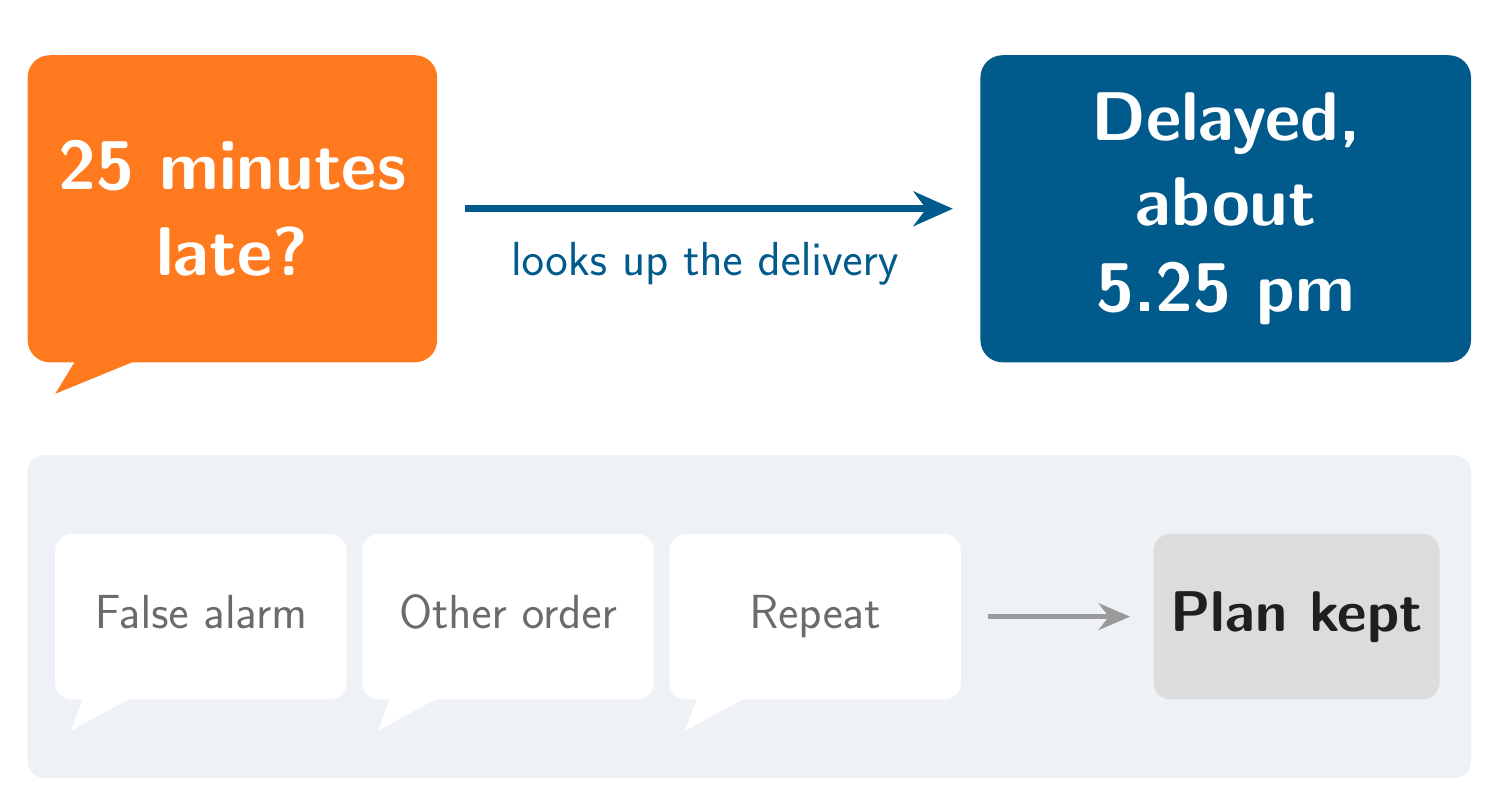
\begin{tikzpicture}[x=1cm, y=1cm, line join=round]
  \def\W{18.33}\def\H{9.53}
  \useasboundingbox (0,0) rectangle (\W,\H);
  % ------------------------------------------------------------ top row, the look-up
  \def\yt{\H}\def\rh{4.6}
  \fill[accent, rounded corners=8pt] (0,\yt-0.35) rectangle (5.2,\yt-\rh+0.35);
  \fill[accent] (0.6,\yt-\rh+0.36) -- (0.35,\yt-\rh-0.05) -- (1.35,\yt-\rh+0.36) -- cycle;
  \node[text=white, align=center, text width=4.6cm, font=\fontsize{26}{31}\selectfont\bfseries]
    at (2.6,\yt-\rh/2) {25 minutes late?};
  % the arrow, with the mark and the label
  \draw[umbblue, line width=2.4pt, -{Stealth[length=5mm,width=4.4mm]}] (5.55,\yt-\rh/2) -- (11.75,\yt-\rh/2);
  \node[text=umbblue, font=\fontsize{36}{36}\selectfont] at (8.6,\yt-\rh/2+1.0) {\markcheck};
  \node[text=umbblue, font=\fontsize{19}{22}\selectfont] at (8.6,\yt-\rh/2-0.7) {looks up the delivery};
  % the answer
  \fill[umbblue, rounded corners=8pt] (12.1,\yt-0.35) rectangle (\W,\yt-\rh+0.35);
  \node[text=white, align=center, text width=5.8cm, font=\fontsize{26}{31}\selectfont\bfseries]
    at ({(12.1+\W)/2},\yt-\rh/2) {Delayed, about 5.25 pm};
  % ------------------------------------------------------------ bottom row, messages that change nothing
  \fill[ground, rounded corners=6pt] (0,0) rectangle (\W,4.1);
  \foreach \i/\lab in {0/False alarm, 1/Other order, 2/Repeat}{
    \pgfmathsetmacro{\x}{0.35+\i*3.9}
    \fill[white, rounded corners=6pt] (\x,1.0) rectangle (\x+3.7,3.1);
    \fill[white] (\x+0.35,1.01) -- (\x+0.2,0.6) -- (\x+0.95,1.01) -- cycle;
    \node[text=muted, font=\fontsize{18}{21}\selectfont] at (\x+1.85,2.05) {\strut\lab};
  }
  \draw[quiet, line width=1.6pt, -{Stealth[length=4mm,width=3.4mm]}] (12.2,2.05) -- (14.0,2.05);
  \fill[rulegrey!60, rounded corners=6pt] (14.3,1.0) rectangle (\W-0.4,3.1);
  \node[text=ink, font=\fontsize{22}{26}\selectfont\bfseries] at ({(14.3+\W-0.4)/2},2.05) {Plan kept};
\end{tikzpicture}
\end{document}
